% GNUPLOT: LaTeX picture with Postscript
\begingroup
  \makeatletter
  \providecommand\color[2][]{%
    \GenericError{(gnuplot) \space\space\space\@spaces}{%
      Package color not loaded in conjunction with
      terminal option `colourtext'%
    }{See the gnuplot documentation for explanation.%
    }{Either use 'blacktext' in gnuplot or load the package
      color.sty in LaTeX.}%
    \renewcommand\color[2][]{}%
  }%
  \providecommand\includegraphics[2][]{%
    \GenericError{(gnuplot) \space\space\space\@spaces}{%
      Package graphicx or graphics not loaded%
    }{See the gnuplot documentation for explanation.%
    }{The gnuplot epslatex terminal needs graphicx.sty or graphics.sty.}%
    \renewcommand\includegraphics[2][]{}%
  }%
  \providecommand\rotatebox[2]{#2}%
  \@ifundefined{ifGPcolor}{%
    \newif\ifGPcolor
    \GPcolortrue
  }{}%
  \@ifundefined{ifGPblacktext}{%
    \newif\ifGPblacktext
    \GPblacktexttrue
  }{}%
  % define a \g@addto@macro without @ in the name:
  \let\gplgaddtomacro\g@addto@macro
  % define empty templates for all commands taking text:
  \gdef\gplbacktext{}%
  \gdef\gplfronttext{}%
  \makeatother
  \ifGPblacktext
    % no textcolor at all
    \def\colorrgb#1{}%
    \def\colorgray#1{}%
  \else
    % gray or color?
    \ifGPcolor
      \def\colorrgb#1{\color[rgb]{#1}}%
      \def\colorgray#1{\color[gray]{#1}}%
      \expandafter\def\csname LTw\endcsname{\color{white}}%
      \expandafter\def\csname LTb\endcsname{\color{black}}%
      \expandafter\def\csname LTa\endcsname{\color{black}}%
      \expandafter\def\csname LT0\endcsname{\color[rgb]{1,0,0}}%
      \expandafter\def\csname LT1\endcsname{\color[rgb]{0,1,0}}%
      \expandafter\def\csname LT2\endcsname{\color[rgb]{0,0,1}}%
      \expandafter\def\csname LT3\endcsname{\color[rgb]{1,0,1}}%
      \expandafter\def\csname LT4\endcsname{\color[rgb]{0,1,1}}%
      \expandafter\def\csname LT5\endcsname{\color[rgb]{1,1,0}}%
      \expandafter\def\csname LT6\endcsname{\color[rgb]{0,0,0}}%
      \expandafter\def\csname LT7\endcsname{\color[rgb]{1,0.3,0}}%
      \expandafter\def\csname LT8\endcsname{\color[rgb]{0.5,0.5,0.5}}%
    \else
      % gray
      \def\colorrgb#1{\color{black}}%
      \def\colorgray#1{\color[gray]{#1}}%
      \expandafter\def\csname LTw\endcsname{\color{white}}%
      \expandafter\def\csname LTb\endcsname{\color{black}}%
      \expandafter\def\csname LTa\endcsname{\color{black}}%
      \expandafter\def\csname LT0\endcsname{\color{black}}%
      \expandafter\def\csname LT1\endcsname{\color{black}}%
      \expandafter\def\csname LT2\endcsname{\color{black}}%
      \expandafter\def\csname LT3\endcsname{\color{black}}%
      \expandafter\def\csname LT4\endcsname{\color{black}}%
      \expandafter\def\csname LT5\endcsname{\color{black}}%
      \expandafter\def\csname LT6\endcsname{\color{black}}%
      \expandafter\def\csname LT7\endcsname{\color{black}}%
      \expandafter\def\csname LT8\endcsname{\color{black}}%
    \fi
  \fi
  \setlength{\unitlength}{0.0500bp}%
  \begin{picture}(8062.00,6192.00)%
    \gplgaddtomacro\gplbacktext{%
      \csname LTb\endcsname%
      \put(1342,704){\makebox(0,0)[r]{\strut{} 0}}%
      \put(1342,1440){\makebox(0,0)[r]{\strut{} 50000}}%
      \put(1342,2177){\makebox(0,0)[r]{\strut{} 100000}}%
      \put(1342,2913){\makebox(0,0)[r]{\strut{} 150000}}%
      \put(1342,3649){\makebox(0,0)[r]{\strut{} 200000}}%
      \put(1342,4385){\makebox(0,0)[r]{\strut{} 250000}}%
      \put(1474,484){\makebox(0,0){\strut{} 2}}%
      \put(2088,484){\makebox(0,0){\strut{} 2.5}}%
      \put(2703,484){\makebox(0,0){\strut{} 3}}%
      \put(3317,484){\makebox(0,0){\strut{} 3.5}}%
      \put(3932,484){\makebox(0,0){\strut{} 4}}%
      \put(4546,484){\makebox(0,0){\strut{} 4.5}}%
      \put(5160,484){\makebox(0,0){\strut{} 5}}%
      \put(5775,484){\makebox(0,0){\strut{} 5.5}}%
      \put(6389,484){\makebox(0,0){\strut{} 6}}%
      \put(6521,704){\makebox(0,0)[l]{\strut{} 0}}%
      \put(6521,1440){\makebox(0,0)[l]{\strut{} 5000}}%
      \put(6521,2177){\makebox(0,0)[l]{\strut{} 10000}}%
      \put(6521,2913){\makebox(0,0)[l]{\strut{} 15000}}%
      \put(6521,3649){\makebox(0,0)[l]{\strut{} 20000}}%
      \put(6521,4385){\makebox(0,0)[l]{\strut{} 25000}}%
      \put(176,2765){\rotatebox{-270}{\makebox(0,0){\strut{}Wall Time ($\mu$sec), naive}}}%
      \put(7554,2765){\rotatebox{-270}{\makebox(0,0){\strut{}Wall Time ($\mu$sec), controlled}}}%
      \put(3931,154){\makebox(0,0){\strut{}Skew}}%
    }%
    \gplgaddtomacro\gplfronttext{%
      \csname LTb\endcsname%
      \put(5534,6019){\makebox(0,0)[r]{\strut{}NaiveRank $mr\hat{\sigma}=$1.542 $avg\hat{\sigma}=$0.32}}%
      \csname LTb\endcsname%
      \put(5534,5799){\makebox(0,0)[r]{\strut{}NaiveSelect $mr\hat{\sigma}=$1.821 $avg\hat{\sigma}=$0.5}}%
      \csname LTb\endcsname%
      \put(5534,5579){\makebox(0,0)[r]{\strut{}ControlledNodeRank $mr\hat{\sigma}=$13.628 $avg\hat{\sigma}=$3.29}}%
      \csname LTb\endcsname%
      \put(5534,5359){\makebox(0,0)[r]{\strut{}ControlledNodeSelect $mr\hat{\sigma}=$4.984 $avg\hat{\sigma}=$1.8}}%
    }%
    \gplbacktext
    \put(0,0){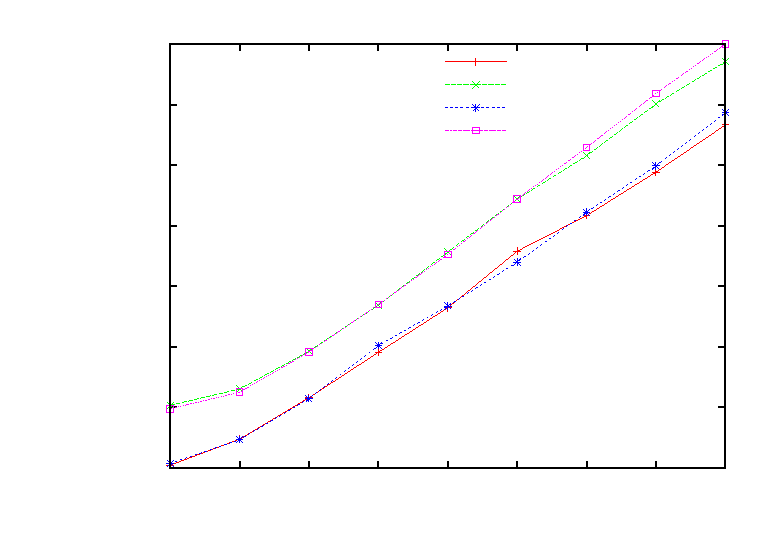
\includegraphics{naiveRankSelectSkewRunningTime}}%
    \gplfronttext
  \end{picture}%
\endgroup
